\section{GENESIS: automated pulse programme creation}
\label{sec:noah__genesis}

In this section, I discuss the development of the GENESIS (GENEration of Supersequences In Silico) website (\cref{fig:genesis_frontpage}): as the name suggests, it automatically generates pulse programmes for arbitrary NOAH supersequences.
The website also provides extensive instructions on acquiring and processing NOAH data.
Although this may at first glance appear slightly out of chronological order, in that the paper\autocite{Yong2022AC} was published later than much of the other work in this chapter, an early version of the GENESIS tool was in fact created much earlier (by July 2020).

The present version of GENESIS is available at \url{https://nmr-genesis.co.uk}.

\begin{figure}[!ht]
    \centering
    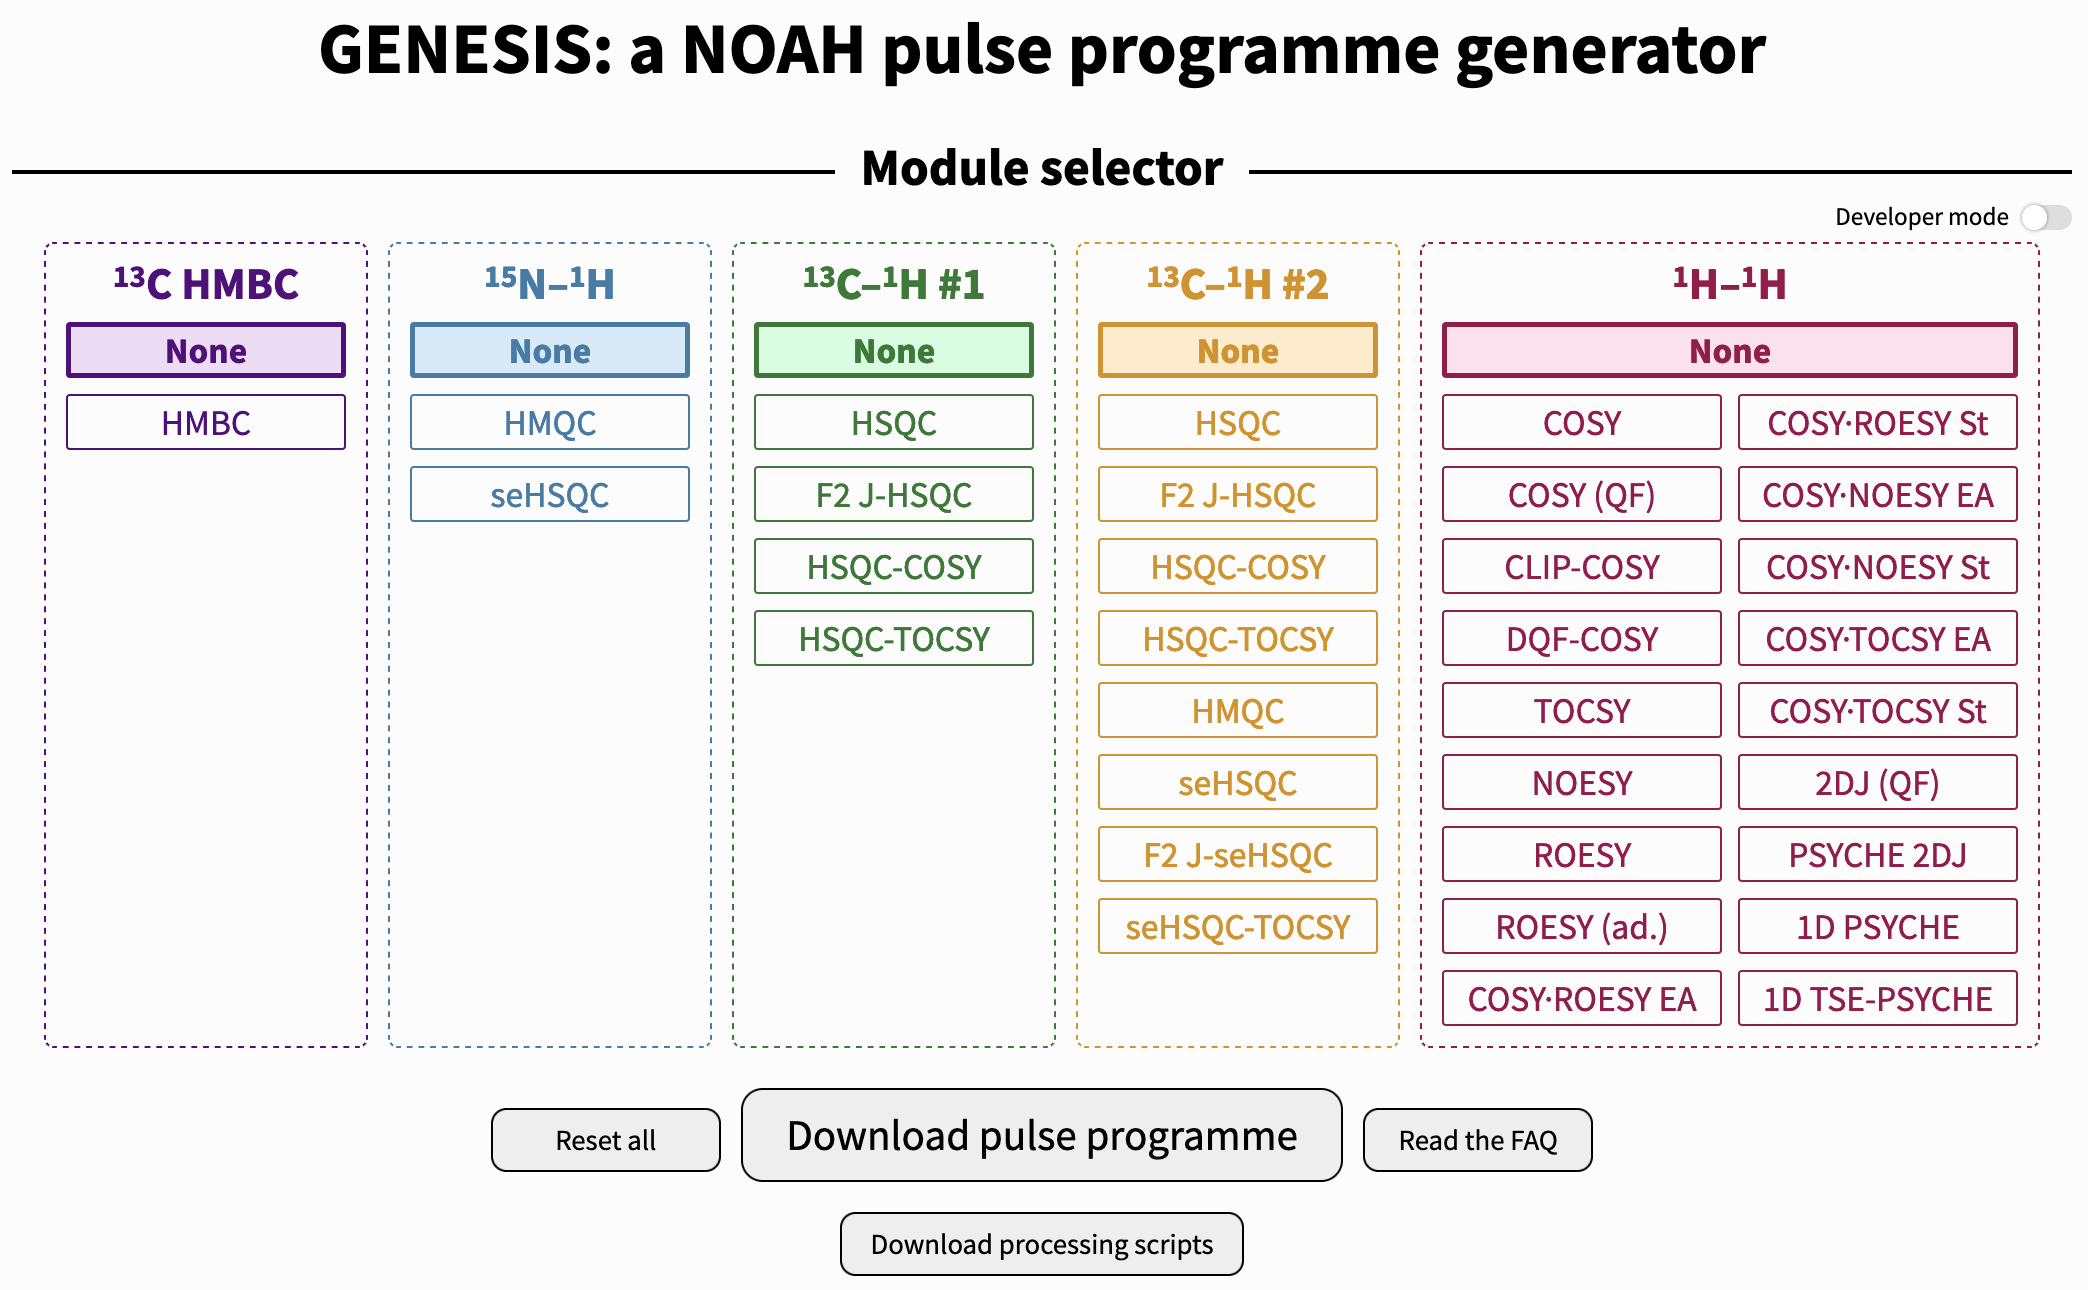
\includegraphics[draft=false,width=0.9\textwidth]{noah/genesis_frontpage.png}%
    \caption[Front page of the GENESIS website]{
        The front page of the GENESIS website (\url{https://nmr-genesis.co.uk}), as of 10 September 2022.
    }
    \label{fig:genesis_frontpage}
\end{figure}

\subsection{Motivation}
\label{subsec:noah__genesis_motivation}

From the preceding discussion in \cref{sec:noah__introduction}, it is clear that modules which use different magnetisation pools can be combined almost at will.
It does not matter \textit{what} modules they are, merely what magnetisation pools they consume (and preserve).
Thus, for example, the \noah{S,C} supersequence can in fact be generalised to any \magn{C} module plus any \magnnot{C} module.

Very broadly speaking, we may define a generic supersequence as having any or all of the following:

\begin{itemize}
    \item a HMBC module, which actually uses \magn{!X} magnetisation but can be placed at the front as discussed in the \noah{B,S,C} example above;
    \item a \magn{N} module;
    \item one or more \magn{C} modules (it is possible to partition the \magn{C} magnetisation pool between two modules, as will be discussed in \cref{subsec:noah__hsqctocsy});
    \item one or more \magn{!X} modules which consume bulk magnetisation.
\end{itemize}

In the first NOAH paper in 2017\autocite{Kupce2017ACIE}, a total of 285 `viable' supersequences were already listed.
If we further take into account some of the new modules which were developed over the course of my DPhil (\cref{sec:noah__modules}), this generic structure means that there are over 4000 viable supersequences.%
\footnote{This is also ignoring the `parallel' supersequences, which are discussed in \cref{sec:noah__parallel}. The support for parallel supersequences in GENESIS is not complete: integrating these fully would require substantial changes to the user interface, which I have not had time to do.}
(`Non-viable' sequences would be those which have undesirable drawbacks: for example, wrongly ordered modules like in a \noah{C,S} supersequence.)

Despite this, \textit{only around 45 pulse programmes} have been published in \textit{all} the NOAH papers to date, or submitted to the Bruker User Library.
Traditionally, NOAH pulse programmes must be written by hand, which is a laborious and fairly error-prone process made worse by the sheer length of these experiments.
Doing this for thousands of supersequence is clearly impractical; furthermore, each time a new module is developed, or an old module is improved, updating every relevant supersequence would itself already be a mammoth task.
This explains why---although the NOAH concept provides a clear blueprint for how supersequences may be constructed---there is still a huge gap between theory and practice.

To bridge this gap, I turned towards the \textit{programmatic} generation of pulse programmes.%
\footnote{This is actually a bit of a lie: GENESIS was initially created for my own convenience. Throughout this chapter, I have had to perform many comparisons of different supersequences, and this tool spared me from having to write everything by hand (and---more often than not---subsequently discover mistakes which invalidated the results). Of course, it soon became apparent that this could be much more widely applicable.}
This not only allows for existing supersequences to be generated at will, but also provides an easy way for updates to be rapidly disseminated to the NMR community.
Furthermore, a website can serve as a `one-stop' shop where---after downloading pulse programmes---users may download the associated NOAH processing scripts and also access instructions on how to run NOAH experiments.
This information did already exist, but was scattered across several different websites and/or journal supplementary information documents, and would have been needlessly confusing to a new user (not to mention the different versions of scripts available in different publications).


\subsection{Implementation details}
\label{subsec:noah__genesis_implementation}

I will now describe a few features of GENESIS pulse programmes, as well as how these are implemented.
The GENESIS code is written in TypeScript; during deployment, this is compiled to JavaScript, which can then be directly executed in the client's web browser.
No server-side code is required, meaning that the GENESIS web page is actually a static site (it is currently hosted using GitHub Pages).

\subsubsection{Overview}

The algorithm used for pulse programme construction can loosely be separated into three parts:
\begin{enumerate}
    \item the \textit{preamble}, which consists of everything up until the beginning of the actual pulse sequence (the \texttt{ze} command). This includes header comments (for the user) as well as definitions of parameters, such as delays and pulse widths;
    \item the \textit{main section}, which contains the actual pulse sequence;
    \item the \textit{epilogue}, which contains phase cycle information as well as footer comments describing each parameter. Instructions for generating shaped pulses using Bruker's WaveMaker software are also included here.
\end{enumerate}

\todo{FIG - breakdown of pulse sequence}

The construction of the preamble and main section is largely accomplished through the collation of module-specific information, the most important of which are:
\begin{itemize}
    \item information about the module itself, which go into the header comments;
    \item parameter definitions, which are collated to form the preamble. Duplicates must be removed here to avoid errors; and
    \item the pulse programmes themselves, which are directly concatenated to form the main section.
\end{itemize}
These, as well as other smaller bits of information (e.g.\ relevant citations, appropriate processing scripts), are stored within \texttt{NOAHModule} objects.
Each distinct module corresponds to one such object.
Therefore, if one wants to add a new module to GENESIS, most of the work can be completed by simply defining a new \texttt{NOAHModule} object: no changes to the algorithm itself are needed.%
\footnote{The website layout must also be changed so that users can actually select the new module.}

Since NOAH experiments are 2D experiments, there is one additional complication: the pulse programme must contain appropriate looping statements, together with pulse phase and delay incrementation, in order to correctly generate the indirect dimension.
In many existing NOAH pulse programmes, looping in 2D experiments was written using the equivalent of \texttt{for} loops (\todo{listing}).
Although this suffices for the vast majority of supersequences, the implementation of parallel supersequences was particularly problematic, as an additional nested loop must be added.
Thus, I opted to only use \textit{one} loop, and to control the phase and delay incrementation using modular arithmetic: the outcome is entirely equivalent, but there is no need to adjust the loop statement itself when switching between linear and parallel supersequences.

\todo{listings to illustrate the above}

To put the epilogue together, the pulse programme constructed so far is scanned for pulse phases, shaped pulses, and all other parameters.
Using predefined lookup tables, GENESIS then outputs pulse phase definitions, WaveMaker directives (where appropriate), and comments containing textual descriptions of each parameter.
These comments are mostly cosmetic, but are very useful to the user as they are displayed in the \texttt{ased} screen when setting up an experiment.
Finally, instructions for automatic processing of the NOAH data (explained in \cref{subsec:noah__genesis_motivation}) are added to the bottom, together with the version number and a timestamp (for reproducibility purposes).

\subsubsection{Module choice}

Developer mode

\subsubsection{Parameter standardisation}
\subsubsection{Parameter descriptions}
\subsubsection{Tests}
\subsubsection{How smart is GENESIS?}



\subsection{Processing improvements}
\label{subsec:noah__genesis_processing}
